\section{Cross teams process}
In the first weeks of the semester, all groups had to define the process for \gls{G19}, which resulted in a manual\cite{processManual}, written by \gls{SMT}.
The manual defines the practices and process to be followed by the groups. The decisions described in the following, are defined in the manual. 

The GIRAF coordinator arranged a presentation by Anton Christensen, a student of \gls{G18}.
Christensen described how his year had worked in teams that focused on one part of the system, for example the server. 
He described that this way of dividing the work made the developers very dependent on each other, and this had been an issue for the groups. 
We decided to use another method, where the teams are \Glspl{fullStack}. This means, that the teams work on whole user stories rather than on a specific areas. 

\subsection{Process activities}
There are three different \glspl{skillGroup}, namely frontend, backend and server. These groups makes it possible for all \glspl{devTeam} to gain knowledge in the specific areas of the system.
In the \gls{SOS} process, the activities resembles the normal each group represents a team member in the normal Scrum process.

Using the \gls{SOS} process, we can think of each \gls{devTeam} as being a person in regular Scrum. Internally, each \gls{devTeam} has its own process. 
There are four sprints planned, and in the following is described the activities in each sprint:

\begin{itemize}
    \item \Gls{SOSSprintPlanning}
    \item \Gls{SOSStandUp}
    \item \Gls{skillGroup} Meetings
    \item \Gls{ReleasePreparation}
    \item \Gls{SOSSprintRetrospective}
    \item \Gls{SOSSprintReview}
    \item Release Party
\end{itemize}

The SOS process is graphically represented in \autoref{fig:SOSProcess}. Here, the circles represent an activity. They are placed in chronological order on the line, with the ones on the loop repeating. The stickmen represents a group member with a role. The "any member" role represents all of the group members. If when one stickman is placed in an activity, it means that one person from the group has to attend. 

One of each \gls{skillGroup} character are placed in the \gls{skillGroup} meeting activity. This means that they attend the \gls{skillGroup} meetings as representatives of their \glspl{devTeam}.
If an activity does not contain a stickman, it is attended by every member of the teams.

\begin{figure}[h]
    \begin{center}
        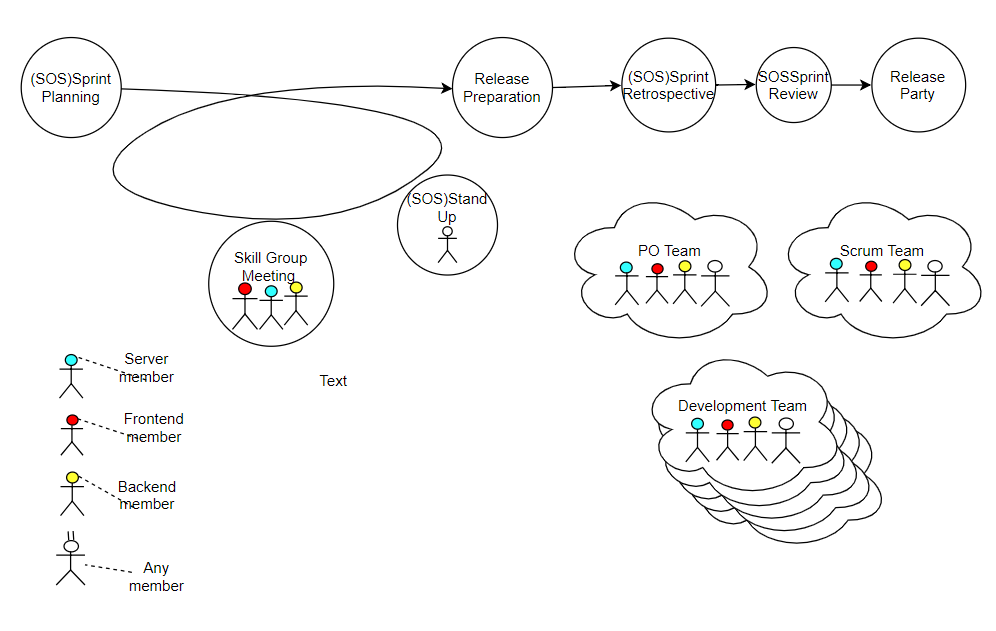
\includegraphics[width=0.95\textwidth]{figures/SOSProcess}
    \end{center}
    \caption{Representation of the \gls{SOS} process.}
    \label{fig:SOSProcess}
\end{figure}

The seven groups are represented with a cloud. \gls{SOS} only describes the process between \glspl{devTeam}. It is up to each group to define their own process, as long as it fits within the \gls{SOS} guidelines. 

\subsubsection{Activities}
The following part describes each of the activities.

\Gls{SOSSprintPlanning} is a meeting held on the first day of each sprint where all members of \Gls{G19} attend. Before the \Gls{SOSSprintPlanning}, the \gls{POT} has prepared user stories for the sprint backlog, and the purpose of the sprint. \gls{POT} presents these stories to the \glspl{devTeam}s, and they choose which user stories they want to implement, and consense with \gls{PO}. When the \glspl{devTeam} has found some tasks appropriate for them, they should leave the meeting.
This is then presented for all \glspl{devTeam}, and the teams will then choose which user stories to implement, and estimate the chosen stories. 
The members of the \gls{POT} is available for questions, and needs to accept the other groups chosen stories and estimates. 
When the \glspl{devTeam} has found a number of tasks appropriate for them, they should leave the meeting. 
 
\Gls{SOSStandUp} is a meeting that is held one to three times a week. The purpose of this meeting, is to share the progress and challenges between the teams, so the different teams knows how the system is progressing, and can help each other with questions. 
Each group should send as few as possible people to answer the questions. The meeting should not take more than 15 minutes. 

The \Gls{skillGroup} meetings, are held so the members of each \gls{skillGroup} is kept up to date with what is going on in his part of the system. The goal is to have at least one meeting every week. 

\Gls{ReleasePreparation} covers four days before the end of each sprint. Here, the system are made ready for release, and the new features and changes are validated and verified. 

\Gls{SOSSprintReview} is held in the end of a sprint. Here only one group member may attend. In this meeting, each group representative talkes about what that group has been working on during the sprint. The progress on all user stories is evaluated. 

In the \gls{SOSSprintRetrospective} the development process is evaluated. Here all group members participates. Beforehand, the groups have to reflect on how they feel the \gls{SOS} process has been. There are formed small group containing approximately one member from each group. The members discuss how they interpret their groups findings. The feedback is collected, and the ideas is voted on. 

The last activity, the Release Party, is held as the last thing in each Sprint. The purpose here is to enhance the \glspl{devTeam} feeling of ownership of the GIRAF project, and to enhance communication between the \glspl{devTeam}. If the different groups want to, they can present the work they have done during the Sprint.

\subsection*{Practices and standards} 
In the manual, some standards and practices the \glspl{devTeam} has to follow. These fit into the following categories:
\begin{itemize}
    \item Coding standards
    \item Documentation standards
    \item Version control
    \item Code review
\end{itemize}

The coding standards involves naming conventions, descriptions and a few other aspects. This is done so the code is easier to read for people that need to get familiar with the system, mainly the following years \glspl{devTeam}, because we found it hard to get to know the system when it was made by a lot of different people, with a lot of different coding standards.
It was also decided, that the \glspl{devTeam} should document the implemented components, their responsibility and how it interacts with other components. A good documentation of this makes it easier for following years. 
Last year, the project and repository was moved to Gitlab that now takes care of the version control. In the beginning of this semester our team moved it to Github. This is documented in section \todo{Ref to sction}. The workflow of the project is done using GitFlow Workflow. In the manual is described the rules for using branches. 
The point of the code review is to make sure that all code committed by the \glspl{devTeam} follows the coding standards. When a Team try to commit code, two people from different groups have to review it. They have to go through a checklist, to see if everything is alright. 

If a member of a team finds an issue in the program, he can make an issue report. This makes it possible to document errors systematically, without the \glspl{team} having to fix it themselves. If a \gls{team} however finds it important to introduce a new task to the product backlog, the team can issue a task creation request. The \gls{POT} then decides if they find it relevant to have in the product backlog. 

The process between the \gls{G19} \glspl{devTeam} is defined in the manual. This process will be evaluated at each \gls{SOSSprintRetrospective}, and changed as needed. It is designed to make the collaboration between the \glspl{team} run as smoothly as possible, without interfering with the \glspl{team} internal processes.  
